%! TEX root = ../main.tex
\documentclass[main]{subfiles}

\begin{document}
\setcounter{chapter}{2} % 章番号を3に設定する
\setcounter{page}{9} % ページ番号を9に設定する
\chapter{有限オートマトン}

本章では\textbf{有限オートマトン}と呼ばれる言語認識機械モデルを紹介し,正規表現で表現できる任意の言語はある有限オートマトンで認識できることを示す.さらに,この逆もいえることも示す.すなわち,有限オートマトンで認識できる任意の言語はある正規表現で表現できることを示し,正規表現で表現できる言語クラスと有限オートマトンで認識できる言語クラスが等しいことを述べる.

\section{決定性有限オートマトン(DFA)}

\begin{mdframed}[
    linewidth=1pt,
    linecolor=black,
    backgroundcolor=white,
    shadow=true,
    shadowsize=4pt,
    shadowcolor=black
]
\noindent 状態集合 $Q$,アルファベット $\Sigma$,遷移関数 $\delta : Q \times \Sigma \rightarrow Q$,初期状態 $s \in Q$,受理(終了)状態 $F \subseteq Q$ から定義される $(Q,\Sigma,\delta,s,F)$ を\textbf{決定性有限オートマトン(deterministic finite automaton: DFA)}と呼ぶ.
\end{mdframed}

\ \\
$\Sigma$上の文字列 $x = x_0 x_1 \cdots x_{n-1}$ に対して,$p_0 = s$, $p_{i+1} = \delta(p_i,x_i)$ $(0 \leq i \leq n - 1)$,$p_n \in F$ であるような状態列 $p_0, p_1, \ldots, p_n$ が存在するとき,この DFA は文字列 $x$ を\textbf{受理する}という.DFA が受理するすべての文字列からなる集合(言語)を $L$ とするとき,この DFA は $L$ を\textbf{認識する}という.

\begin{tcolorbox}[
  enhanced,
  coltitle=black,
  attach boxed title to top left={xshift=3mm, yshift=-\tcboxedtitleheight/2},
  colback=white,
  title=DFA の例:,
  boxed title style={size=small,colframe=white,colback=white}
]
\small
\textbf{例1}\\
$Q = \{q_0, q_1, q_2\}$\\
$\Sigma = \{\mathtt{a,b}\}$\\[-14pt]
\begin{tabular}{c|cc}
$\delta$ & $\mathtt{a}$ & $\mathtt{b}$ \\
\hline
$q_0$ & $q_1$ & $q_0$ \\
$q_1$ & $q_1$ & $q_2$ \\
$q_2$ & $q_2$ & $q_2$ \\
\end{tabular}
\hspace{5mm} $\Leftrightarrow$
\begin{minipage}{0.45\textwidth}
  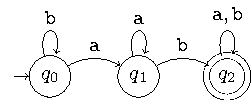
\includegraphics{figures/dfa1.pdf}\\[2mm]
  \small{正規表現 \texttt{b*aa*b} が表す言語\\
  $= \{\mathtt{a}\text{ と }\mathtt{b}\text{ がこの順に現れる文字列}\}$ を認識}
\end{minipage}\\[-20pt]

$s = q_0$\\
$F = \{q_2\}$

\textbf{例2}\\
$Q = \{q_0, q_1\}$\\
$\Sigma = \{\mathtt{a,b}\}$\\[-14pt]
\begin{tabular}{c|cc}
$\delta$ & $\mathtt{a}$ & $\mathtt{b}$ \\
\hline
$q_0$ & $q_0$ & $q_1$ \\
$q_1$ & $q_1$ & $q_1$ \\
\end{tabular}
\hspace{5mm} $\Leftrightarrow$ 
\begin{minipage}{0.45\textwidth}
  
  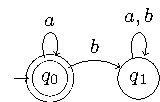
\includegraphics{figures/dfa2.pdf}\\[2mm]
  \small{認識される言語は?}
\end{minipage}\\[-20pt]

$s = q_0$\\
$F = \{q_0\}$

\textbf{例3}\\
$Q = \{q_0, q_1, q_2\}$\\
$\Sigma = \{\mathtt{a,b}\}$\\[-14pt]
\begin{tabular}{c|cc}
$\delta$ & $\mathtt{a}$ & $\mathtt{b}$ \\
\hline
$q_0$ & $q_1$ & $q_2$ \\
$q_1$ & $q_2$ & $q_0$ \\
$q_2$ & $q_2$ & $q_2$ \\
\end{tabular}
\hspace{5mm} $\Leftrightarrow$ 
\begin{minipage}{0.45\textwidth}
  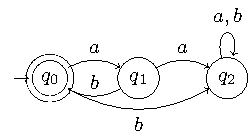
\includegraphics{figures/dfa3.pdf}\\[2mm]
  \small{認識される言語は?}
\end{minipage}\\[-20pt]

$s = q_0$\\
$F = \{q_0\}$
\end{tcolorbox}

\end{document}